% This is samplepaper.tex, a sample chapter demonstrating the
% LLNCS macro package for Springer Computer Science proceedings;
% Version 2.20 of 2017/10/04
%
\documentclass[runningheads]{llncs}
%
\usepackage{graphicx}
\graphicspath{ {./images/} }
\usepackage[utf8]{inputenc}
\usepackage[spanish,es-nodecimaldot]{babel}
\usepackage[spanish, fixlanguage]{babelbib}
\bibliographystyle{splncs04}
% Used for displaying a sample figure. If possible, figure files should
% be included in EPS format.
%
% If you use the hyperref package, please uncomment the following line
% to display URLs in blue roman font according to Springer's eBook style:
% \renewcommand\UrlFont{\color{blue}\rmfamily}

\begin{document}
%
\title{Consejo de embajadores}
\subtitle{Una variación del Naming Game basado en comunidades}
%
%\titlerunning{Abbreviated paper title}
% If the paper title is too long for the running head, you can set
% an abbreviated paper title here
%
\author{Diego de Jesús Isla López y
Saul Ivan Rivas Vega}
%
% First names are abbreviated in the running head.
% If there are more than two authors, 'et al.' is used.
%
\institute{Universidad Nacional Autónoma de México, Ciudad Universitaria, Ciudad de México, México\\
\email{\{diego.isla,saul.ivan.rivas.vega\}@comunidad.unam.mx}}
%
\maketitle              % typeset the header of the contribution
%
\begin{abstract}
El Naming Game es una simulación basada en agentes los cuales con un protocolo de comunicación y una memoria buscan llegar a un acuerdo sobre que única palabra almacenar para nombrar a un objeto. En el presente trabajo extendemos las características del diseño original propuesto por Baronchelli, con el propósito de reportar y analizar las diferencias en los parámetros de estudio durante la simulación. Se llevaron a cabo una serie de experimentos por cada combinación posible dentro de un espacio reducido de valores y la media de resultados son los tomados en cuenta para el análisis. Los resultados son congruentes con los reportes de Baronchelli, además de que se puede observar comportamientos especiales.
\keywords{Naming Game  \and Comunicación \and Agentes \and Inteligencia Artificial \and Simulación.}
\end{abstract}
%
%
%
\section {Introducción}
Se han realizado trabajos con experimentos basados en la hipótesis de que el lenguaje es un sistema adaptativo que se forma así mismo a través de un proceso cultural auto-organizado~\cite{Baronchelli_2006}.

Los juegos del lenguaje fueron propuestos por primera vez en las investigaciones filosóficas de Ludwig Wittgenstein en 1967~\cite{as474369}. Su modelo consiste en considerar a un constructor y a un asistente con distintas herramientas y recursos los cuales el constructor debía solicitar al asistente, lo cual llevaba a comunicarse en un lenguaje primitivo. Sin embargo, Wittgenstein no creía que así era como se comportaba el lenguaje en el mundo real. Lo que el pensaba era que podían reconocerse particularidades de la lingüística que si se asemejan al mundo real.

Posteriormente se realizaron implementaciones de variada complejidad como lo son: \textit{Naming Games}~\cite{RePEc:wsi:acsxxx:v:01:y:1999:i:04:n:s021952599800020x}, \textit{Guessing Games}~\cite{Baronchelli_2006}, \textit{Descripting Games}~\cite{Baronchelli_2006}, etc.
\section{Antecedentes}
El trabajo propuesto en Naming Games~\cite{Baronchelli_2006} inspiró el trabajo de Baronchelli~\cite{Baronchelli_2006} para desarrollar un modelo de comunicación entre agentes. En dicho modelo se utilizaba el siguiente protocolo de comunicación entre el hablante y el escucha que son 2 agentes seleccionados al azar:
\begin{itemize}
	\item El hablante selecciona un objeto del contexto actual
	\item El hablante toma una palabra de su inventario para referirse al objeto, en caso de no tener una palabra, crea una nueva.
	\item El hablante comunica la palabra seleccionada al receptor
	\item Si el escucha tiene en su inventario la palabra que le comunicó el hablante, la comunicación se considera exitosa lo que hace que tanto el hablante como el escucha borren su inventario de palabras para el objeto con excepción de la palabra que ambos conocen.
	\item En caso contrario el escucha almacena en su inventario de palabras la palabra que le comunicó el hablante.
\end{itemize}

\section{Diseño Propuesto}

La variante del \textit{naming game} propuesta consiste en tener comunidades con un número uniforme de miembros. Cada comunidad utiliza un conjunto de reglas para generar palabras diferentes con las cuales designarán a cada uno de los objetos. Cada comunidad decidirá la palabra que le asignará a cada objeto y una vez que todas han llegado a un consenso, los embajadores de cada comunidad se reúnen y entre todos presentan las palabras de sus comunidades y votan las palabras que usarán de ahora en adelante. Una vez que se deciden las palabras finales, los embajadores regresan a sus respectivas comunidades y enseñan las palabras a los demás miembros.\\
Las etapas en el modelo propuesto se pueden visualizar mejor en la figura \ref{fig0}.
\begin{figure}
	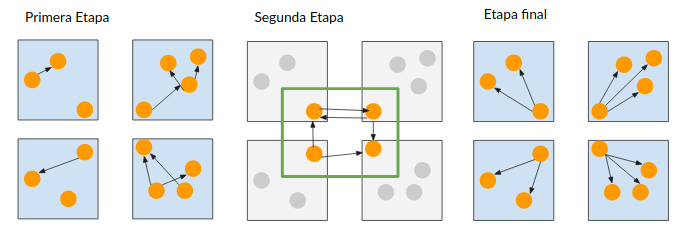
\includegraphics[width=\textwidth]{modelo1.png}
	\caption{Etapas en el modelo.}
	\label{fig0}
\end{figure}

\subsection{Protocolos de comunicación}

Se tienen tres protocolos de comunicación uno por cada etapa del sistema:
\begin{enumerate}
	\item Comunicación entre miembros de una misma comunidad.
	\item Comunicación entre embajadores.
	\item Comunicación del embajador con el resto de su comunidad.
\end{enumerate}
\subsubsection{Primera Etapa}
\paragraph{Comunicación entre miembros de una comunidad}
En esta etapa del sistema las comunicaciones se realizan solamente entre miembros de una misma comunidad y termina hasta que todas las comunidades converjan internamente.
Se sigue el siguiente protocolo de comunicación:
\begin{enumerate}
	\item Tomar 1 comunidad aleatoriamente que no haya convergido internamente aún.
	\item Seleccionar aleatoriamente al agente que escucha y el agente que habla.
	\item Seleccionar el objeto aleatoriamente.
	\item Si el hablante no tiene palabras en su memoria, crea una con base en su regla de generación y la almacena con frecuencia = 1.
	\item El hablante toma la palabra con mayor frecuencia en su memoria.
	\item Si el escucha no conoce la palabra la almacena con una frecuencia = 1.
	\item Si el escucha si conoce la palabra aumenta en 1 su frecuencia y reduce por un factor de olvido (16, suelo) las demás palabras en su memoria.
	\item Si alguna palabra llega a 0 se elimina de su memoria. 
\end{enumerate}

\subsubsection{Segunda Etapa}
En esta etapa del sistema las comunicaciones se realizan solamente entre los embajadores. Existe exactamente un embajador por comunidad, y este puede ser cualquier miembro de la comunidad puesto que todos terminaron con la misma lista de palabras. Comienzan las comunicaciones al finalizar la etapa anterior y terminan hasta que todos los embajadores conozcan la palabra de los demás embajadores.
Se sigue el siguiente protocolo de comunicación:
\begin{enumerate}
	\item El embajador de cada comunidad puede ser cualquiera, se toma al primero de cada comunidad.
	\item Se fuerza la comunicación de todos los embajadores como hablante con cada uno de los otros embajadores como escuchas con cada uno de los objetos.
	\item En cada una de las comunicaciones el embajador hablante comunica la única palabra que tiene actualmente en su memoria.
	\item El escucha evalúa la preferencia por la nueva palabra y si la prefiere en lugar de su palabra actual, la reemplaza, y en caso contrario, la ignora.
	\item Posterior a que todos los embajadores se hayan comunicado y escogieran su palabra preferida, vuelven a comunicarse entre todos.
	\item El hablante escoge su palabra que seleccionó como favorita.
	\item Si el escucha si conoce la palabra aumenta en 1 su frecuencia, en caso contrario la agrega con frecuencia = 1.
	\item Todos los embajadores borran todas las palabras de su memoria, con excepción de la palabra más frecuente en el consejo.
\end{enumerate}
\subsubsection{Tercera Etapa}
Esta es la etapa final del sistema en la que solamente los embajadores propagan la lista de palabras que se obtuvo del consejo y los agentes dentro de la comunidad solo reemplazan la lista que tenían con la del embajador. Las comunicaciones solo se llevan a cabo con el embajador como el hablante y los demás agentes de su comunidad como oyentes. Terminan las comunicaciones cuando todos los agentes de todas las comunidades terminan con la misma lista de palabras.
Se sigue el siguiente protocolo de comunicación:
\begin{enumerate}
	\item El embajador de cada comunidad Comunica su palabra de cada objeto a un miembro de su comunidad con quien no se haya comunicado aún.
	\item El escucha reemplaza la palabra para cada objeto con la que le comunica el embajador.
\end{enumerate}

\subsection{Generación de palabras}
Existe un diccionario inicial de sílabas tomadas a partir de concatenar las vocales con cada una de las consonantes del alfabeto. Una \textit{regla de generación} consiste en una tupla $(A,cantidad\_s,separador)$ en donde $A$ es un subconjunto del diccionario de sílabas, $cantidad\_s$ es un entero positivo que determina la cantidad de sílabas que se usarán para formar la palabra y el $separador$ es un elemento del diccionario el cual se coloca entre cada sílaba que se agrega a la palabra durante su formación.\\
Tomando la regla $(\{"ke", "li"\}, 3, "pa")$, puede formarse la palabra \textit{kepakepalipa}.\\
Cada comunidad cuenta con su propia regla de generación determinada antes del inicio de la primera etapa.
\subsection{Evaluación de preferencia}
Entre embajadores, se evalúa la preferencia al recibir una palabra de una comunidad ajena. Esto se hace comparando la palabra recibida con respecto a las reglas de generación del receptor. Por el momento se hace una evaluación simple, para saber que tanto prefiere una palabra un agente se cuentan cuantas sílabas de la regla de generación se encuentran en la palabra, mientras mas sílabas tenga en común mayor será su preferencia por la palabra.
Por ejemplo si un agente tiene en su comunidad la regla de generación $(\{"ke", "li"\}, 3, "pa")$ va a tener una preferencia por la palabra \textit{sigalite} con valor a $1$ puesto que solo tienen en común la sílaba \textit{li}, ahora si tomamos en cuenta la palabra \textit{lilireke}, tendrá una preferencia con valor igual a $3$ puesto que comparten \textit{li} y esta presente 2 veces, y además comparten la sílaba \textit{ke}.
\subsection{Convergencia}
La convergencia la definimos como el momento en que todos los agentes en todas las comunidades tienen la misma palabra para referirse a cada objeto, es decir tienen la misma lista de palabras.
\pagebreak
\section{Experimentos}
Los parámetros que tomamos en cuenta para los experimentos son: La cantidad de agentes totales ($N$), la cantidad de objetos ($O$), y la cantidad de comunidades ($C$). Los agentes son distribuidos equitativamente en las comunidades. En la sección de resultados mostramos los promedios de 100 ejecuciones del programa que tiene algunos de los posibles valores que se muestran en el cuadro \ref{tab0}. 
\begin{table}[h]
	\centering
	\caption{Distintos valores para los experimentos.}\label{tab0}
	\begin{tabular}{|l|l|}
		\hline
		Parámetro &  Valores  \\
		\hline
		N &  50, 100, 200 \\
		\hline
		O &  4, 8, 16 \\
		\hline
		C &  4, 8, 16 \\
		\hline
	\end{tabular}
\end{table}
\section{Resultados}
\subsection{50 agentes en 4 comunidades con 4 objetos}
Descripción.
\begin{figure}[h]
	\centering
	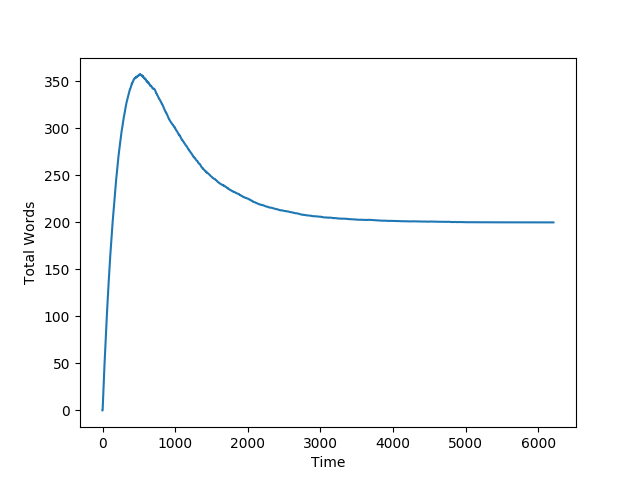
\includegraphics[width=0.65\textwidth]{Figure_111_TotalWords.png}
	\caption{Número de palabras totales.}
	\label{fig_000}
\end{figure}
\begin{figure}[h]
	\centering
	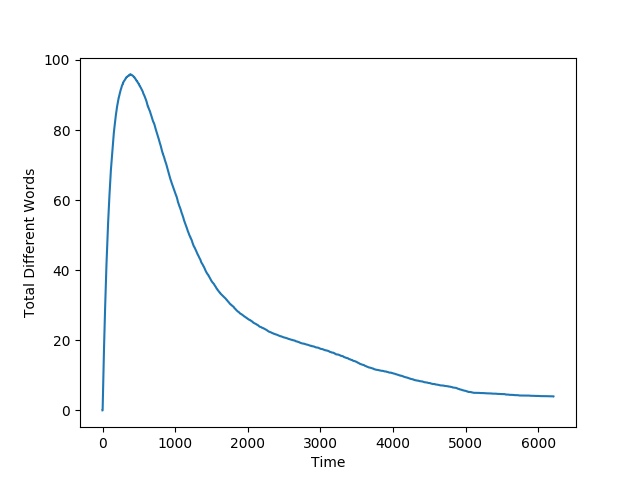
\includegraphics[width=0.65\textwidth]{Figure_111_TotalDifferentWords.png}
	\caption{Número de palabras diferentes totales.}
	\label{fig_001}
\end{figure}
\pagebreak
\\
\subsection{50 agentes en 16 comunidades con 4 objetos}
Descripción.
\begin{figure}[h]
	\centering
	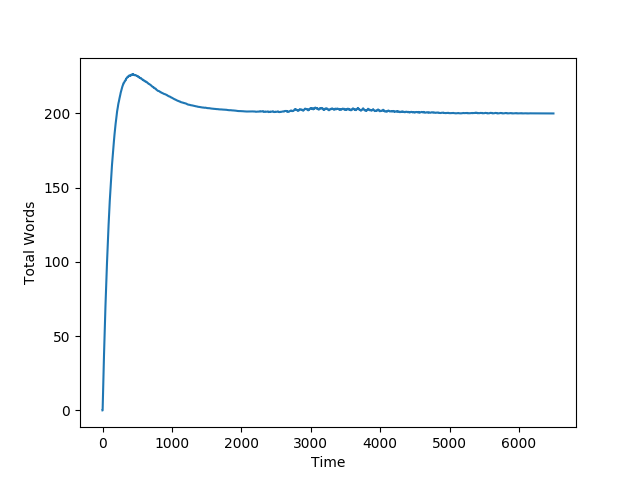
\includegraphics[width=0.65\textwidth]{Figure_113_TotalWords.png}
	\caption{Número de palabras totales.}
	\label{fig_002}
\end{figure}
\begin{figure}[h]
	\centering
	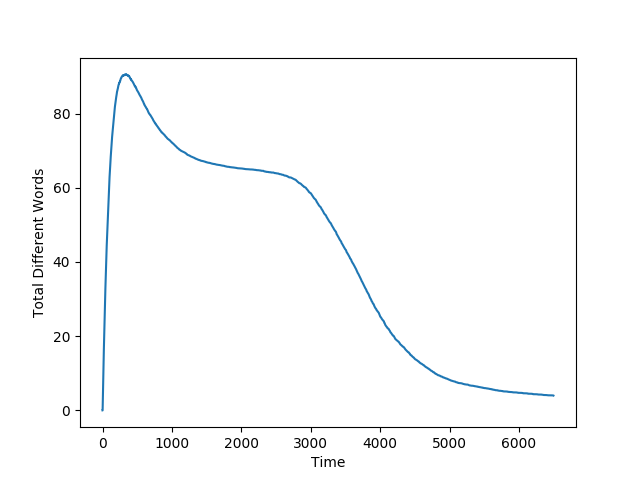
\includegraphics[width=0.65\textwidth]{Figure_113_TotalDifferentWords.png}
	\caption{Número de palabras diferentes totales.}
	\label{fig_003}
\end{figure}
\pagebreak
\\
\subsection{50 agentes en 4 comunidades con 16 objetos}
Descripción.
\begin{figure}[h]
	\centering
	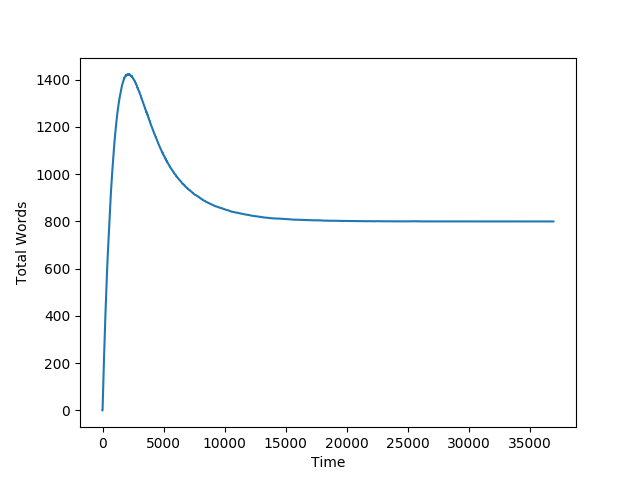
\includegraphics[width=0.65\textwidth]{Figure_311_TotalWords.png}
	\caption{Número de palabras totales.}
	\label{fig_004}
\end{figure}
\begin{figure}[h]
	\centering
	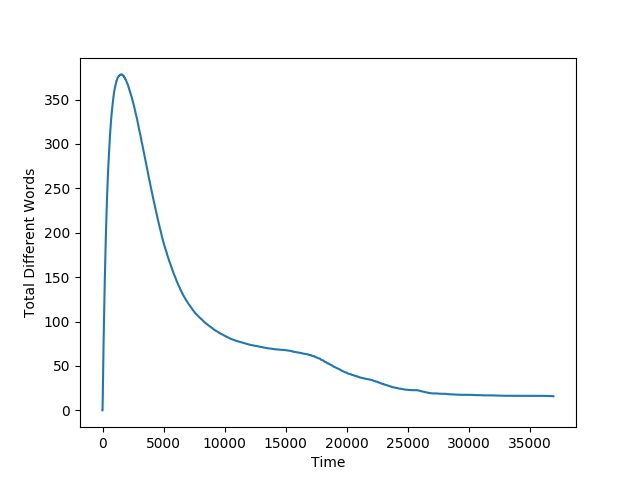
\includegraphics[width=0.65\textwidth]{Figure_311_TotalDifferentWords.png}
	\caption{Número de palabras diferentes totales.}
	\label{fig_005}
\end{figure}
\pagebreak
\\
\subsection{200 agentes en 16 comunidades con 16 objetos}
Descripción.
\begin{figure}[h]
	\centering
	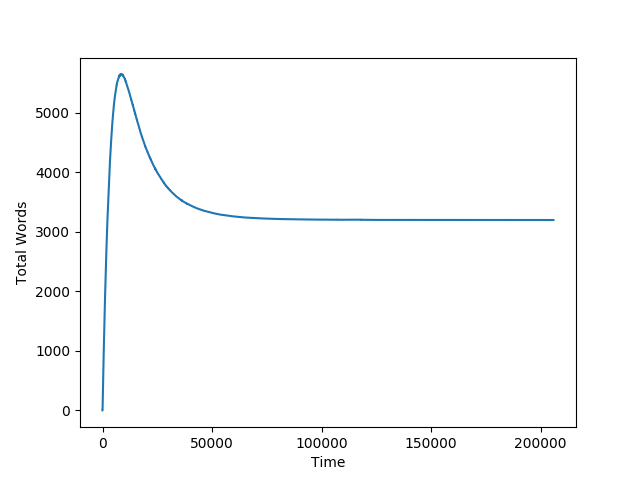
\includegraphics[width=0.65\textwidth]{Figure_333_TotalWords.png}
	\caption{Número de palabras totales.}
	\label{fig_006}
\end{figure}
\begin{figure}[h]
	\centering
	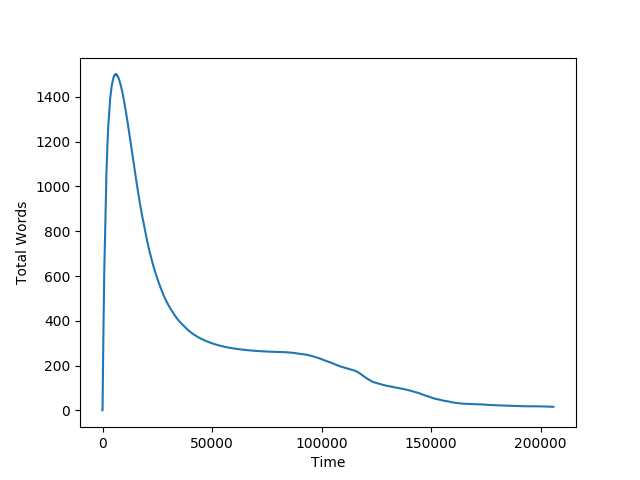
\includegraphics[width=0.65\textwidth]{Figure_333_TotalDifferentWords.png}
	\caption{Número de palabras diferentes totales.}
	\label{fig_007}
\end{figure}
\\
\subsection{Tablas de resultados}
\paragraph{}Descripción.
\begin{table}[h]
	\centering
	\caption{Resultados con 4 Comunidades y 4 objetos, variando N.}\label{tab1}
	\begin{tabular}{|c|c|c|c|c|c|}
		\hline
		N &  T conv & T max Words & Max Words & max dif Words & T conv / T max  \\
		\hline
		50 & 4154.72 &   527.76 & 366.98 & 96.8 & 8.0205 \\
		\hline
		100 & 9799.31 &   1255.67 & 891.11 & 193.89 & 7.8966\\
		\hline
		200 & 22140.05 &  2868.27 & 2148.05 & 392.86 & 7.7545 \\
		\hline
	\end{tabular}
\end{table}
\paragraph{}Descripción.
\begin{table}[h]
	\centering
	\caption{Resultados con 8 Comunidades y 4 objetos, variando N.}\label{tab2}
	\begin{tabular}{|c|c|c|c|c|c|}
		\hline
		N &  T conv & T max Words & Max Words & max dif Words & T conv / T max  \\
		\hline
		50 & 4154.72 &   527.76 & 366.98 & 96.8 & 8.0205 \\
		\hline
		100 & 9799.31 &   1255.67 & 891.11 & 193.89 & 7.8966\\
		\hline
		200 & 22140.05 &  2868.27 & 2148.05 & 392.86 & 7.7545 \\
		\hline
	\end{tabular}
\end{table}
\section{Discusión y Conclusiones}
\paragraph{Impacto del número  de objetos}
El número de objetos hace aumentar el tiempo de convergencia. Se observa que el tiempo de convergencia es proporcional conforme aumenta el número de objetos. Aumenta el valor del Tiempo de Convergencia sobre el Tiempo con el número máximo de palabras.
\paragraph{Impacto de variaciones en comunidades}
El número de comunidades no afecta al tiempo de convergencia, puesto que se ocupa una distribución equitativa. Aumenta de manera significativa el valor del Tiempo de Convergencia sobre el Tiempo con el número máximo de palabras.
\paragraph{Impacto de variación de agentes}
El tiempo de convergencia con respecto a los agentes y objetos, es proporcional. Disminuye el valor del Tiempo de Convergencia sobre el Tiempo con el número máximo de palabras.
\paragraph{Preservación de propiedades del algoritmo original}
Se observa que los resultados obtenidos son congruentes con las observaciones de Baronchelli.
\paragraph{Consideraciones futuras}
\begin{itemize}
	\item Probar con reglas más robustas de generación de palabras.
	\item Tener una base mayor de reglas diferentes y probar diferentes combinaciones.
	\item Una evaluación de preferencia que involucre otros factores de la regla de generación resultante en el punto anterior.
	\item Una variación con el factor de olvido.
	\item Reglas auxiliares para la comunicación entre los embajadores.
\end{itemize}
%
% ---- Bibliography ----
%
% BibTeX users should specify bibliography style 'splncs04'.
% References will then be sorted and formatted in the correct style.
%
% \bibliographystyle{splncs04}
% \bibliography{mybibliography}
%
\bibliography{main}
\end{document}
